\documentclass[12pt]{article}
\usepackage[utf8]{inputenc}
%\usepackage[T1]{fontenc}
%\usepackage{dejavu}

\usepackage{listings}
\usepackage{amsfonts}
\usepackage{fancyhdr}
\usepackage{comment}
\usepackage{graphicx}
\usepackage[letterpaper, top=2.5cm, bottom=2.5cm, left=2.2cm, right=2.2cm]{geometry}
%\renewcommand{\item}[1]{\item \textbf{#1}}
\begin{document}

\begin{center}
%\includegraphics{logo_unah.png}\\
\bfseries{Universidad Nacional Autónoma de Honduras}\\
Facultad de Ingeniería\\
Departamento de Ingeniería en Sistemas\\
\bigskip
\bigskip
IS-611 Redes de Datos 2\\
I PAC 2018

\noindent\rule{\textwidth}{1pt}
\huge{ENRUTAMIENTO DINÁMICO: OSPF}
\noindent\rule{\textwidth}{1pt}
\end{center}
%\title{Resumen sobre Spanning-Tree Protocol}
 %\author{José Mario López}
 %\date{\today}
%\maketitle
 
 \section{Introducción}   
\textbf{OSPFv2} (open shortest path first) fue creado a finales de los 80. Se diseñó para cubrir las necesidades de las grandes redes IP que otros protocolos como RIP no podían soportar, incluyendo VLSM, autenticación de origen de ruta, convergencia rápida, etiquetado de rutas conocidas mediante protocolos de enrutamiento externo y publicaciones de ruta de multidifusión. El protocolo OSPF versión 2 es la implementación más actualizada, aparece especificado en la RFC 2328.\\

OSPF funciona dividiendo una intranet o un sistema autónomoen unidades jerárquicas de menor tamaño. Cada una de estas áreas se enlaza a un área backbone mediante un router de frontera. Todos los paquetes enviados desde una dirección de una estación de trabajo de un área a otra de un área diferente atraviesan el área de backbone, independientemente de la existencia de una conexión directa entre las dos áreas. Aunque es posible el funcionamiento de una red OSPF únicamente con el área backbone, OSPF escala bien cuando la red se subdivide en un número de áreas más pequeñas.\\

OSPF es un protocolo de enrutamiento por estado enlace que a diferencia de RIP e IGRP que publican sus rutas solo a routers vecinos, los routers OSPF envían publicaciones del estado enlace \textbf{LSA} (Link-State Advertisement) a todos los routers pertenecientes a la misma área jerárquica mediante un multicast de IP. La LSA contiene información adicionales necesarios para calcular las bases de datos de la ruta y topología de red. Los routers OSPF acumulan información sobre el estado de enlace y ejecutan el algoritmo \textbf{SPF} (Shortest Path First), también conocido con el nombre de su creador \textbf{dijkstra}, para calcular la ruta más corta a cada nodo.\\

Para determinar qué interfaces reciben las publicaciones de estado de enlace, los routers ejecutan el protocolo OSPF \textbf{hello}. Los routers vecinos intercambian mensajes hello para determinar qué otros routers existen en una determinada interfaz y sirven como mensajes de actividad que indican la accesibilidad de dichos routers.\\

Cuando se detecta un router vecino, se intercambia información de topología OSPF. Cuando los routers están sincronizados, se dice que han formado una adyacencia.\\

Las LSA se envían y reciben solo en adyacencias. La información de la LSA se transporta en paquetes mediante la capa de transporte OSPF que define un proceso fiable de publicación, acuse de recibo y petición para garantizar que la información de la LSA se distribuye adecuadamente a todos los routers de un área.  Los tipos más comunes son los que publican información sobre los enlaces de red conectados de un router y los que publican las redes disponibles fuera de las áreas OSPF.\\

\subsection{Métrica}
 El \textbf{coste} es la métrica utilizada por OSPF. Un factor importante en el intercambio de las LSA es la relativa a la métrica. OSPF calcula el coste mediante la siguiente fórmula:
$$ coste = \frac{100\,000\,000 bps}{Velocidad\_enlace} = \frac{10^8 bps}{Velocidad\_enlace}$$

Si existen varios caminos para llegar al destino con el mismo coste, OSPF efectúa por defecto un balanceo de carga hasta 4 rutas diferentes. Este valor admite hasta 16 rutas diferentes. OSPF calcula el coste de manera acumulativa tomando en cuenta el coste de la interfaz de salida de cada router.

\subsection{Tablas}
\begin{itemize}
\item \textbf{Tabla de vecinos}: contiene la información sobre los vecions con los cuáles se realizan intercambios OSPF.\\
\item \textbf{Tabla de topologías}: mantiene una base de datos de todas las LSA recibidas de toda la red.\\
\item \textbf{Tabla de enrutamiento}: contiene la información necesaria para alcanzar una red de destino.
\end{itemize}

\subsection{Mantenimiento de la base de datos}
Los protocolos vector distancia anuncian rutas hacia los vecinos, pero los protocolos de estado enlace anuncian una lista de todas sus conexiones. Cuando un enlace se cae, se envían LSA (Link-State Advertisement), que son compartidas por los vecions como así también una base topológica \textbf{LSDB} (Link-State Database).  las LSA se identifican con un número de secuencia para reconocer las más recientes, en un ranto de 0x8000 0001 al 0xFFFF FFFF. Cuando los routers convergen tienen la misma LSDB, a partir de ese momento SPF es capaz de determinar la mejor ruta hacia el destino. La tabla de topología es la visión que tiene el router de la red dentro del área en que se encuentra incluyendo además todos los routers\\

La tabla de topología se actualiza por cada una de las LSA que envían cada uno de los routers dentro de la misma área y que todos estos routers comparten la misma base de datos. Si existen inconsistencias en esta base de datos, podrían generarse bucles; el propio router es el encargado de avisar que ha habido algún cambio en informar del mismo.\\

Algunos de éstos pueden ser:
\begin{itemize}
\item Pérdida de conexión física o link en algunas de sus interfaces.
\item No se reciben los hello en el tiempo establecido por sus vecinos.
\item Se recibe un LSA con información de cambios de topología
\end{itemize}

En cualquiera de los tres casos anteriores el router generará una LSA enviando a sus vecinos la siguiente información:
\begin{itemize}
\item Si la LSA es más reciente se añade a la base de datos. Se reenvían a todos los vecinos para que actualicen sus tablas y SPF comienza a funcionar.
\item Si el número de secuencia es el mismo que el que el router ya tiene registrado en la base de datos, ignorará esta actualización.
\item Si el número de secuencia es anterior al que está registrado, el router enviará la versión nueva al router que envió la anterior. De esa forma se asegura que todos los routers poseen la última versión.
\end{itemize}

\subsection{Relación de vecindad}
OSPF establece relaciones con otros routers mediante el intercambio de mensajes hello. Luego del intercambio inicial de estos mensajes, los routers elaboran sus tablas de vecinos, que lista todos los routers que están ejecutando OSPF y están directamente conectados. Los mensajes hello son enviadors con la dirección multicast 224.0.0.5 con una frecuencia en redes tipo broadcast cada 10 segundos, mientras que en las redes non-broadcast, cada 30 segundos.\\

Una vez que los routers hayan intercambiado los paquetes hello, comienzan a intercambiar información acerca de la red y una vez que esa información haya sincronizado, los routers forman adyacencias.\\

Una vez lograda la adyacencia (estado \textbf{full}), las tablas deben mantenerse actualizadas, las LSA son enviadas cuando exista algún cambio o cada 30 segundos como un tiempo de refresco.\\
 
La siguiente lista describe los estados de una relación de vecindad:
\begin{itemize}
\item \textbf{Down}: es el primer estado de OSPF y significa que no se ha escuchado ningún hello de este vecino.\\
\item \textbf{Attempt}: este estado es únicamente para redes NBMA (Multiacceso sin broadcast), durante este estado, el router envía paquetes hello de tipo unicast hacia el vecino aunque no se hayan recibido hello de ese vecino.\\
\item \textbf{Init}: se ha recibido un paquete hello de un vecino pero el ID del router no está listado en ese paquete hello.\\
\item \textbf{2-Way}: se ha establecido una comunicación bidireccional entre dos routers.\\
\item \textbf{Exstart}: una vez elegidos el DR y el BDR, el verdadero proceso de intercambiar información del estado enlace se hace entre los routers y sus DR y BDR.\\
\item \textbf{Exchange}: en este estado los routers intercambian la información de la base de datos.\\
\item \textbf{Loading}: es en este estado cuando se produce el verdadero intercambio de la información de estado de enlace.\\
\item \textbf{Full}: finalmente los routers son totalmente adyacentes, se intercambian las LSA y las bases de datos de los routers están sincronizadas.\\
\end{itemize}

Los mensajes hello se siguen enviando periódicamente para mantener las adyacencias, en el caso de que no se reciban, se dará por perdida dicha adyancencia. Tan pronto como OSPF detecta un problema, modifica las LSA correspondientes y envía actualizaciones a todos los vecinos. Este proceso mejora el tiempo de convergencia y reduce al mínimo la cantidad de información que se envía en la red.

\subsection{Router Designado}
Cuando varios routers están conectados a un segmento de red del tipo broadcast (Ethernet, por ejemplo), uno de estos routers del segmento tomará el control y mantendrá las adyacencias entre todos los routers de ese segmento. Ese router toma el nombre de \textbf{DR} (Designated Router) y será elegido a través de la información que contienen los mensajes hello que se intercambian los routers. Para una eficaz redundancia también se elige un router designado de reserva o \textbf{BDR}. Los DR son creados en enlaces multiacceso debido a que el número de adyacencias incrementaría de manera significativa el tráfico en la red, de esta forma el DR y el BDR establecen adyacencias reduciendo significativamente la cantidad de las mismas.\\

La elección de un router designado (DR) y un router desingado de reserva (BDR) en una topología multiacceso con difusión, cumple los siguientes requisitos:
\begin{itemize}
\item El router con el valor de prioridad más alto es el router designado \textbf{DR}
\item El router con el segundo valor de prioridad más alto es el router designado de reserva \textbf{BDR}
\item El valor predeterminado de la prioridad de OSPF de la interfaz es \textbf{1}. Un router con prioridad 0 no es elegible. En caso de empate, se usa el ID del router.
\item ID de router: es un número de 32 bits que identifica únicamente al router dentro de un sistema autónomo. La dirección IP más alta de una interfaz, se elige por defecto.
\end{itemize}

Los routers que no son DR ni BDR se denominan \textbf{DRother}.

\subsection{Topologías OSPF}
\subsubsection{Multiacceso con difusión}
Dado que el enrutamiento OSPF depende el estado de enlace entre dos routers, los vecinos deben reconocerse entre sí para compartir información. Este proceso se hace por medio del protocolo Hello.\\

Los paquetes se envían cada 10 segundos de manera predeterminada. Para declarar un vecino caído el router espera 4 veces el tiempo del intervalo hello, y se denomina a este, intervalo dead.\\

Los routers en entornos multiacceso, como un entorno Ethernet, deben elegir un router designado (\textbf{DR}) y un \textbf{BDR} para que se representen en la red.\\

Un DR lleva a cabo tareas de envío y sincronización. El BDR solo actuará si el DR falla. Cada router debe establecer una adyacencia con el DR y el BDR.

\begin{figure}[h]
\centering
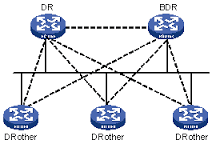
\includegraphics[scale=1.5]{ospf_dr_bdr.png}
\caption{En redes con difusión (broadcast) se lleva a cabo la elección del DR y BDR}
\end{figure}

\subsubsection{NBMA}
No se abordará en la asignatura.

\subsubsection{Punto a Punto}
En redes punto a punto el router detecta dinámicamente a sus vecinos enviando paquetes hello con la dirección de multidifusión 224.0.0.5
\textbf{No se lleva a cabo elección y no existe concepto de DR o BDR}.\\
Los intervalos hello y dead son de 10 y 40, respectivamente.

\begin{figure}[h]
\centering
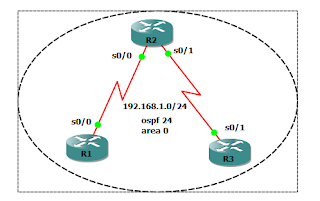
\includegraphics[scale=1]{ospf_ppp.png}
\caption{En redes punto a punto no se lleva a cabo la elección del DR y BDR}
\end{figure}

\subsection{Configuración de OSPF en una sola área}
Para iniciar el proceso de configuración OSPF se debe identificar el número de proceso. Este número tiene significado local y pueden existir varios procesos OSPF en un mismo router, aunque hay que tener en cuenta que cuantos más procesos, más consumo de recursos.  [1]\\

Una vez que el proceso OSPF es habilitado, se debe identificar las interfaces que participarán en el mismo, debiendo tener especial cuidado con la utilizaciòn de la máscara comodín o wildcard (la wildcard se obtiene restando 255 del valor del octeto correpondiente en la máscara de subred, por ejemplo, para la máscara 255.255.255.252 corresponde la wildcard 0.0.0.3) [2]\\

El parámetro \textit{área} asocia las interfaces en un área en particular. El formato del parámetro es un campo de 32 bits en decimal simple o notación decimal punteada.\\

A partir de la indentificación del área comienzan a intercambiarse los hello, se envían las LSA y el conjunto de los routers comienzan a participar en la red. Cuando el router tiene interfaces en diferentes áreas se llama ABR o router de borde.\\

La wildcard permite especificar una red, una subred, una interfaz específica, un rango de interfaces o todas las interfaces que participarán del proceso OSPF. Existen varias formas de utilizar el comando \textit{network} aprovechando la flexibilidad de las wildcard:
\begin{enumerate}
\item Configurando de manera global todas las interfaces.
\item Configurando las redes a las que pertenecen las interfaces. 
\item Configurando las interfaces una a una.
\end{enumerate}

Estas opciones pueden ser aplicables con mayor eficacia según sea el caso. La primera puede ser de rápida configuración pero con el consiguiente riesgo de que alguna interfaz no deseada se filtre en el proceso OSPF. El tercer caso es más trabajoso para el administrador pero más selectivo y seguro.\\

\begin{lstlisting}
[1] Router(config)# router ospf <numero de proceso>
[2] Router(config-router)# network <direccion de red> ...
				... <wildcard> area <numero>
\end{lstlisting}

\begin{figure}[h]
\centering
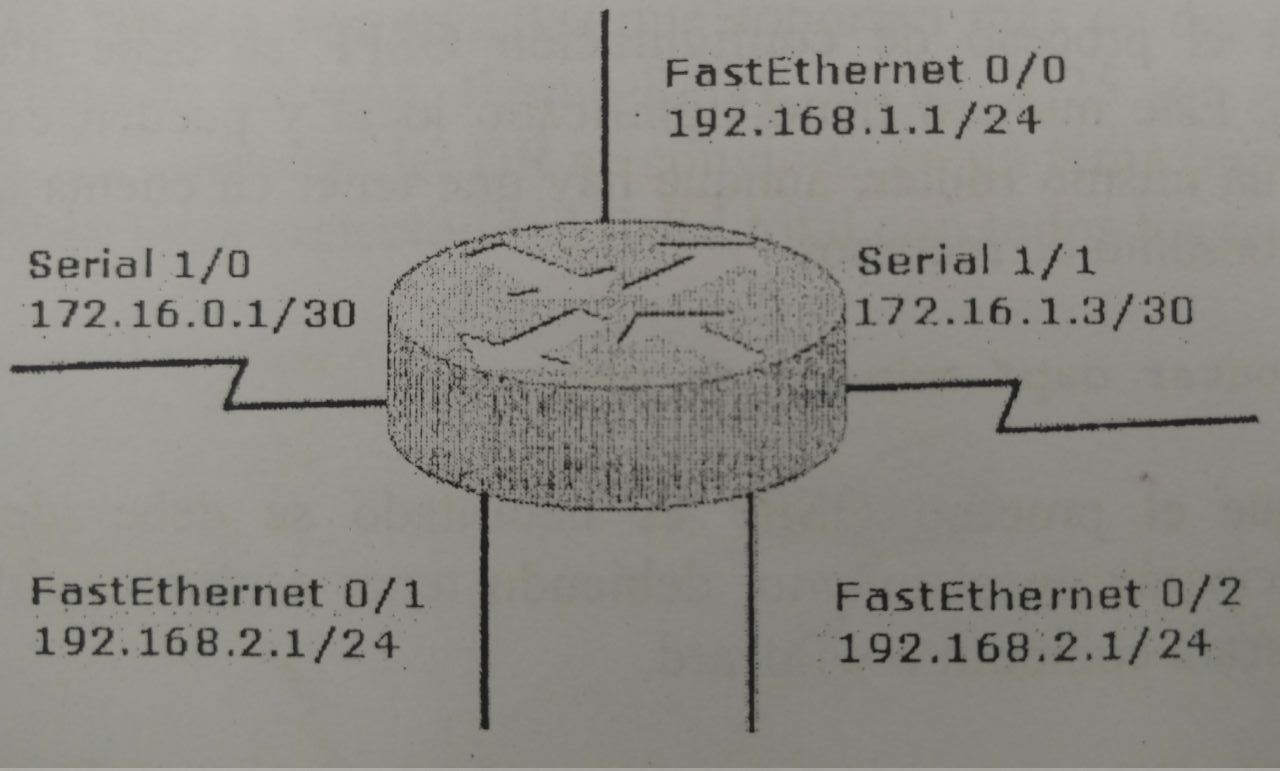
\includegraphics[scale=0.25]{ospf_example_addressing.jpg}
%\caption{En redes punto a punto no se lleva a cabo la elección del DR y BDR}
\end{figure}

Configurando de manera global todas las interfaces:
\begin{lstlisting}
Router(config-router)# network 0.0.0.0 255.255.255.255 area 0
\end{lstlisting}

Configurando las redes a las que pertenecen las interfaces:
\begin{lstlisting}
Router(config-router)# network 172.16.0.0 0.0.255.255 area 0
Router(config-router)# network 192.168.1.0 0.0.0.255 area 0
\end{lstlisting}

Configurando las interfaces una a una:
\begin{lstlisting}
Router(config-router)# network 192.168.1.1 0.0.0.0 area 0
Router(config-router)# network 192.168.2.1 0.0.0.0 area 0
Router(config-router)# network 192.168.3.1 0.0.0.0 area 0
Router(config-router)# network 172.16.0.1 0.0.0.0 area 0
Router(config-router)# network 172.16.1.3 0.0.0.0 area 0
\end{lstlisting}

\subsubsection{Elecciòn del DR y BDR}
La elección del DR y el BDR puede manipularse acorde a las necesidades existentes variando los valores de la prioridad dentro de la interfaz o subinterfaz que participe en el dominio OSPF (rango de 1 a 65535).
\begin{lstlisting}
Router# configure terminal
Router(config)# interface <tipo> <numero>
Router(config-if)# ip ospf priority <1-65535>
\end{lstlisting}

\subsubsection{Cálculo de coste del enlace}
Para modificar el ancho de banda sobre la interfaz, utilice el comando \textbf{bandwith}
\begin{lstlisting}
Router(config)# interface <tipo> <numero>
Router(config-if)# bandwidth 64
\end{lstlisting}

Al utilizar este comando, el valor de ancho de banda se ve afectado de manera lògica, para efectos del cálculo del coste.

\subsubsection{Administración del protocolo Hello}
De manera predeterminada, los paquetes de saludo OSPF (Hello) se envían cada 10 segundos en segmentos multiacceso y punto a punto, y cada 30 segundos en segmentos multiacceso sin broadcast (NBMA).\\

El intervalo muerto (Dead) es el período, expresado en segundos, que el router esperará para recibir un paquete de saludo antes de declarar al vecino desactivado. Cisco utiliza de forma predeterminada cuatro veces el intervalo hello. En el caso de los segmentos multiacceso y punto a punto, dicho período es de 40 segundos. En el caso de las redes NBMA, el intervalo muerto es de 128 segundos.\\

Para configurar los intervalos Hello y Dead en una interfaz, se deben utilizar los siguientes comandos:
\begin{lstlisting}
Router(config-if)# ip ospf hello-interval <segundos>
Router(config-if)# ip ospf dead-interval <segundos>
\end{lstlisting}

\subsubsection{Verificación}
Algunos comandos para la verificaciòn y control de OSPF son:
\begin{itemize}
\item \textbf{show ip route}: muestra la tabla de enrutamiento.
\item \textbf{show ip protocols}: muestra los parámetros del protocolo.
\item \textbf{show ip ospf neighbor}: muestra la información de los vecinos OSPF.
\item \textbf{debug ip ospf events}: muestra adyacencias, DR, broadcasts, etc.
\item \textbf{debug ip ospf packet}: muestra la información de los paquetes de OSPF.
\item \textbf{debug ip ospf hello}: muestra las actualizaciones Hello.
\end{itemize}

\vfill
{\textbf {\normalsize José Mario López}}

{\small Profesor de la asignatura\\}

{\footnotesize 
El contenido fue tomado de Ariganello, Ernesto. Redes Cisco, Guía de estudio para la certificación CCNA Routing y Switching (2014).

De presentarse alguna duda respecto al contenido del resumen, recuerde que puede avocarse al Departamento de Ing. En Sistemas, en hora de consulta de 15:00 – 16:00 de lunes a viernes; o enviar un correo a jmlopezc@unah.edu.hn}

\end{document}